We first discuss our base linear models for the three tasks: Bayesian
$L_2$-regularized linear (for \sts{} and \sas{}) and logistic
(for \asr{}) regression.  We extend these models for (1)
adaptation across different short text similarity domains, and (2)
multitask learning of short text similarity (\sts{}), short answer scoring
(\sas{}) and answer sentence ranking (\asr{}).


\subsection{Base Models}
\label{section:approach-base-models}


In our base models (\Cref{figure:base-models}), the feature vector
$\boldsymbol{f}$ combines with the feature weight vector
$\boldsymbol{w}$ (including a bias term $w_0$) to form predictions.
Each parameter $w_i \in \boldsymbol{w}$ has its own zero-mean Gaussian
prior with its standard deviation $\sigma_{w_i}$ distributed uniformly
in $[0, m_{\sigma_w}]$, the covariance matrix $\boldsymbol{\Sigma}_w$
is diagonal, and the zero-mean prior $L_2$ regularizes the model.

\begin{figure}[t]
    \centering
    \begin{subfigure}[b]{0.5\textwidth}
        \centering
        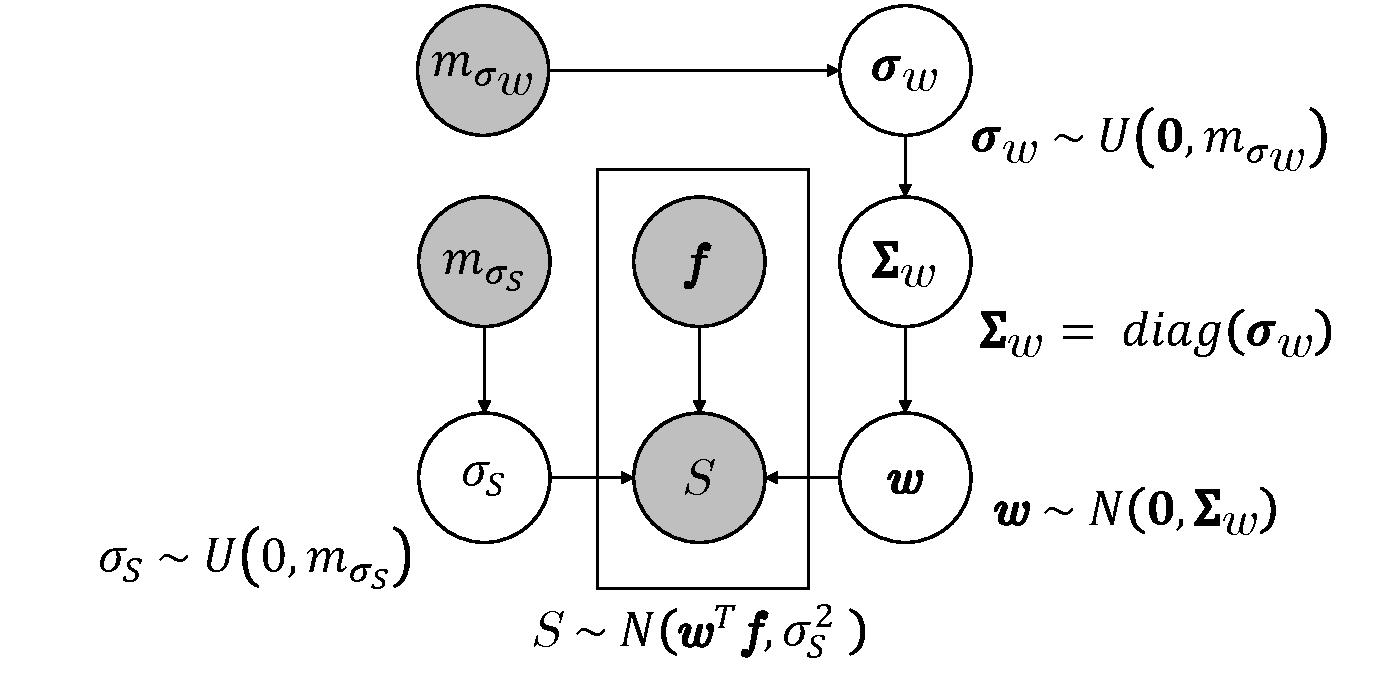
\includegraphics[scale=0.35]{2016_naacl_stsdomain/figures/sts_sas_model.pdf}
        \caption{Bayesian ridge regression for \sts{} and \sas{}.}
        \label{figure:sts-sas-model}
    \end{subfigure}
    \newline
    \newline
    \begin{subfigure}[b]{0.5\textwidth}
        \centering
        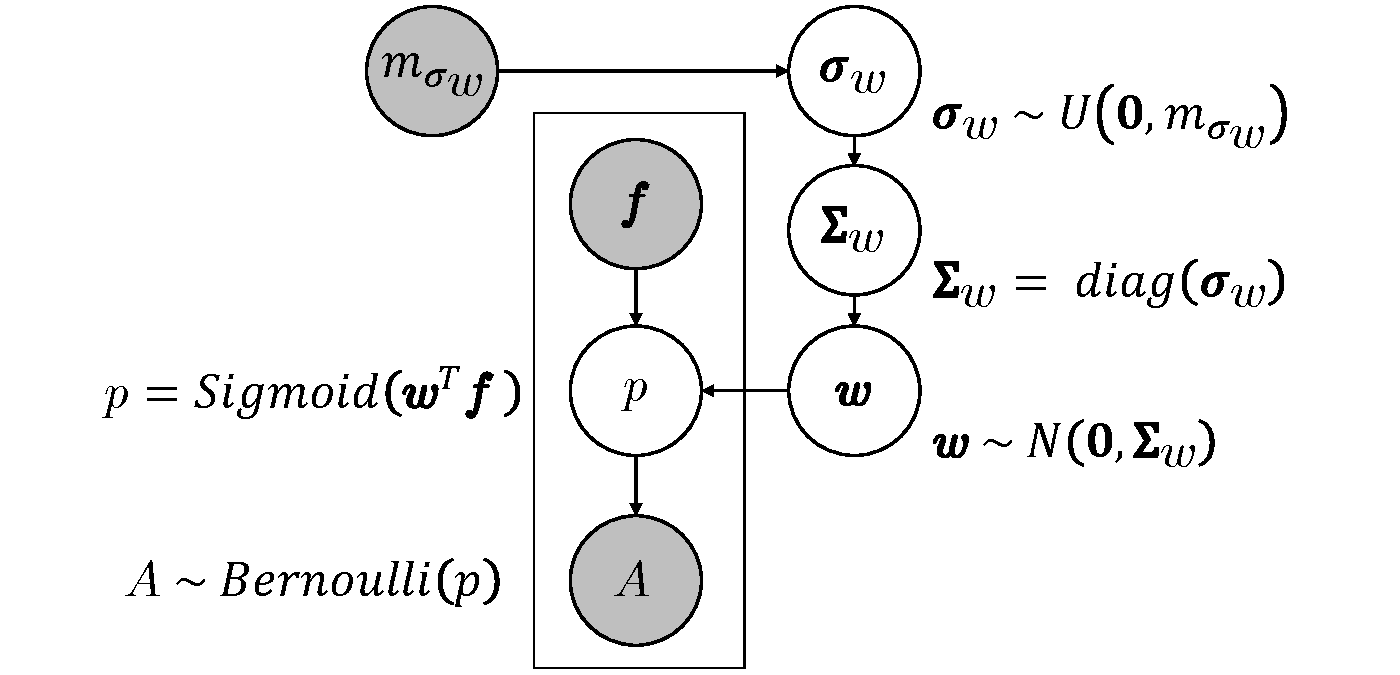
\includegraphics[scale=0.35]{2016_naacl_stsdomain/figures/asr_model.pdf}
        \caption{Bayesian logistic regression for \asr{}.}
        \label{figure:asr-model}
    \end{subfigure}
    \newline
    \caption{Base models for \sts{}, \sas{} and \asr{}.  Plates represent
      replication across sentence pairs.  Each model learns weight vector
      $\boldsymbol{w}$.  For \sts{} and \sas{}, the real-valued output~$S$
      (similarity or student score) is normally distributed around the
      weight-feature dot product $\boldsymbol{w}^T\boldsymbol{f}$.  For \asr{},
      the sigmoid of this dot product is the Bernoulli prior for the binary
      output $A$, relevance of the question's answer candidate.}
    \label{figure:base-models}

    
    
\end{figure}

In the linear model (\Cref{figure:sts-sas-model}), $S$ is the output
(similarity score for \sts{}; answer score for \sas{}) and is normally
distributed around the dot product
$\boldsymbol{w}^T\boldsymbol{f}$.  The model error $\sigma_S$ has a
uniform prior over a prespecified range $[0, m_{\sigma_S}]$.  In the
logistic model (\Cref{figure:asr-model}) for \asr{}, the probability
$p$ that the candidate sentence answers the question, is (1) the sigmoid of
$\boldsymbol{w}^T\boldsymbol{f}$, and (2) the Bernoulli prior of $A$,
whether or not the candidate answers the question.

The common vectors $\boldsymbol{w}$ and $\boldsymbol{f}$ in these models enable
joint parameter learning and consequently multitask learning (\Cref{section:approach-mtl}).


\subsection{Adaptation to \sts{} Domains}
\label{section:approach-da}


Domain adaptation for the linear model (\Cref{figure:sts-sas-model})
learns a separate weight vector $\boldsymbol{w}_d$ for each
domain $d$ (i.e., applied to similarity computations for test pairs in
domain $d$) alongside a common, global domain-agnostic weight
vector $\boldsymbol{w}_*$, which has a zero-mean Gaussian prior and
serves as the Gaussian prior mean for each
$\boldsymbol{w}_d$.
\Cref{figure:da-sts-model} shows the model.
Both $\boldsymbol{w}_*$ and
$\boldsymbol{w}_d$ have hyperpriors identical to $\boldsymbol{w}$ in
\Cref{figure:sts-sas-model}.\footnote{Results do not improve with
  individual domain-specific instances of $\sigma_S$ and
  $\boldsymbol{\sigma}_w$, consistent with \newcite{finkel-09} for
  dependency parsing and named entity recognition.}

\begin{figure}[t]
\centering
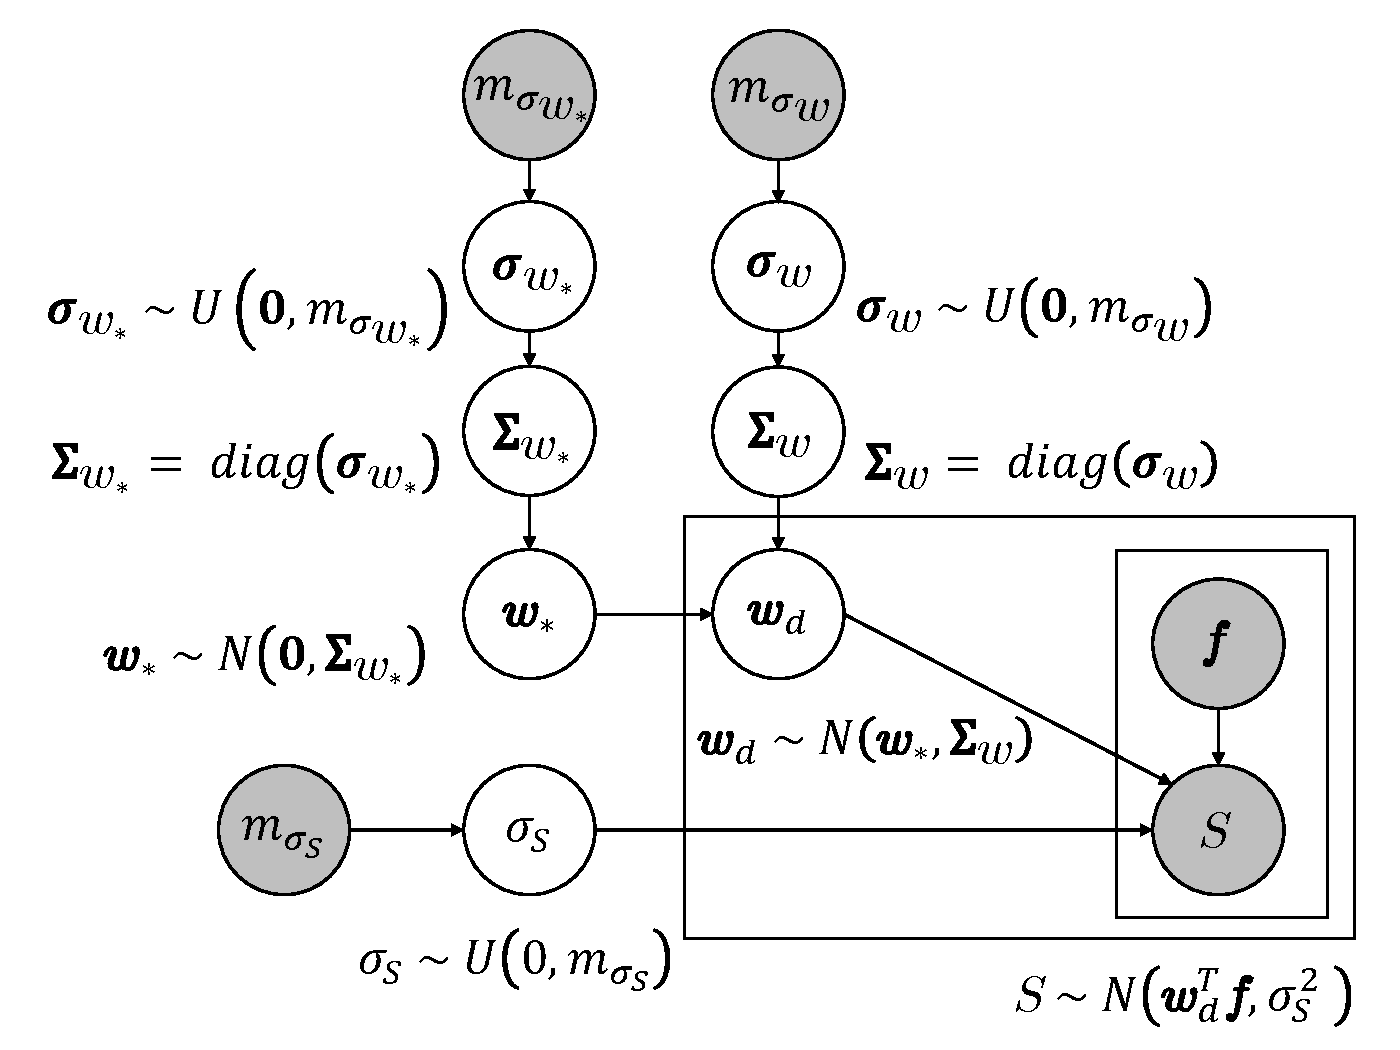
\includegraphics[trim={6mm 0 0 0},clip,scale=0.35]{2016_naacl_stsdomain/figures/da_sts_model_practical.pdf}
\caption{Adaptation to different \sts{} domains. The outer plate represents replication across
domains. Joint learning of a global weight vector $\boldsymbol{w}_*$ along with individual
domain-specific vectors $\boldsymbol{w}_d$ enables inductive transfer among domains.}
\label{figure:da-sts-model}
\end{figure}

\begin{figure*}[ht]
\centering
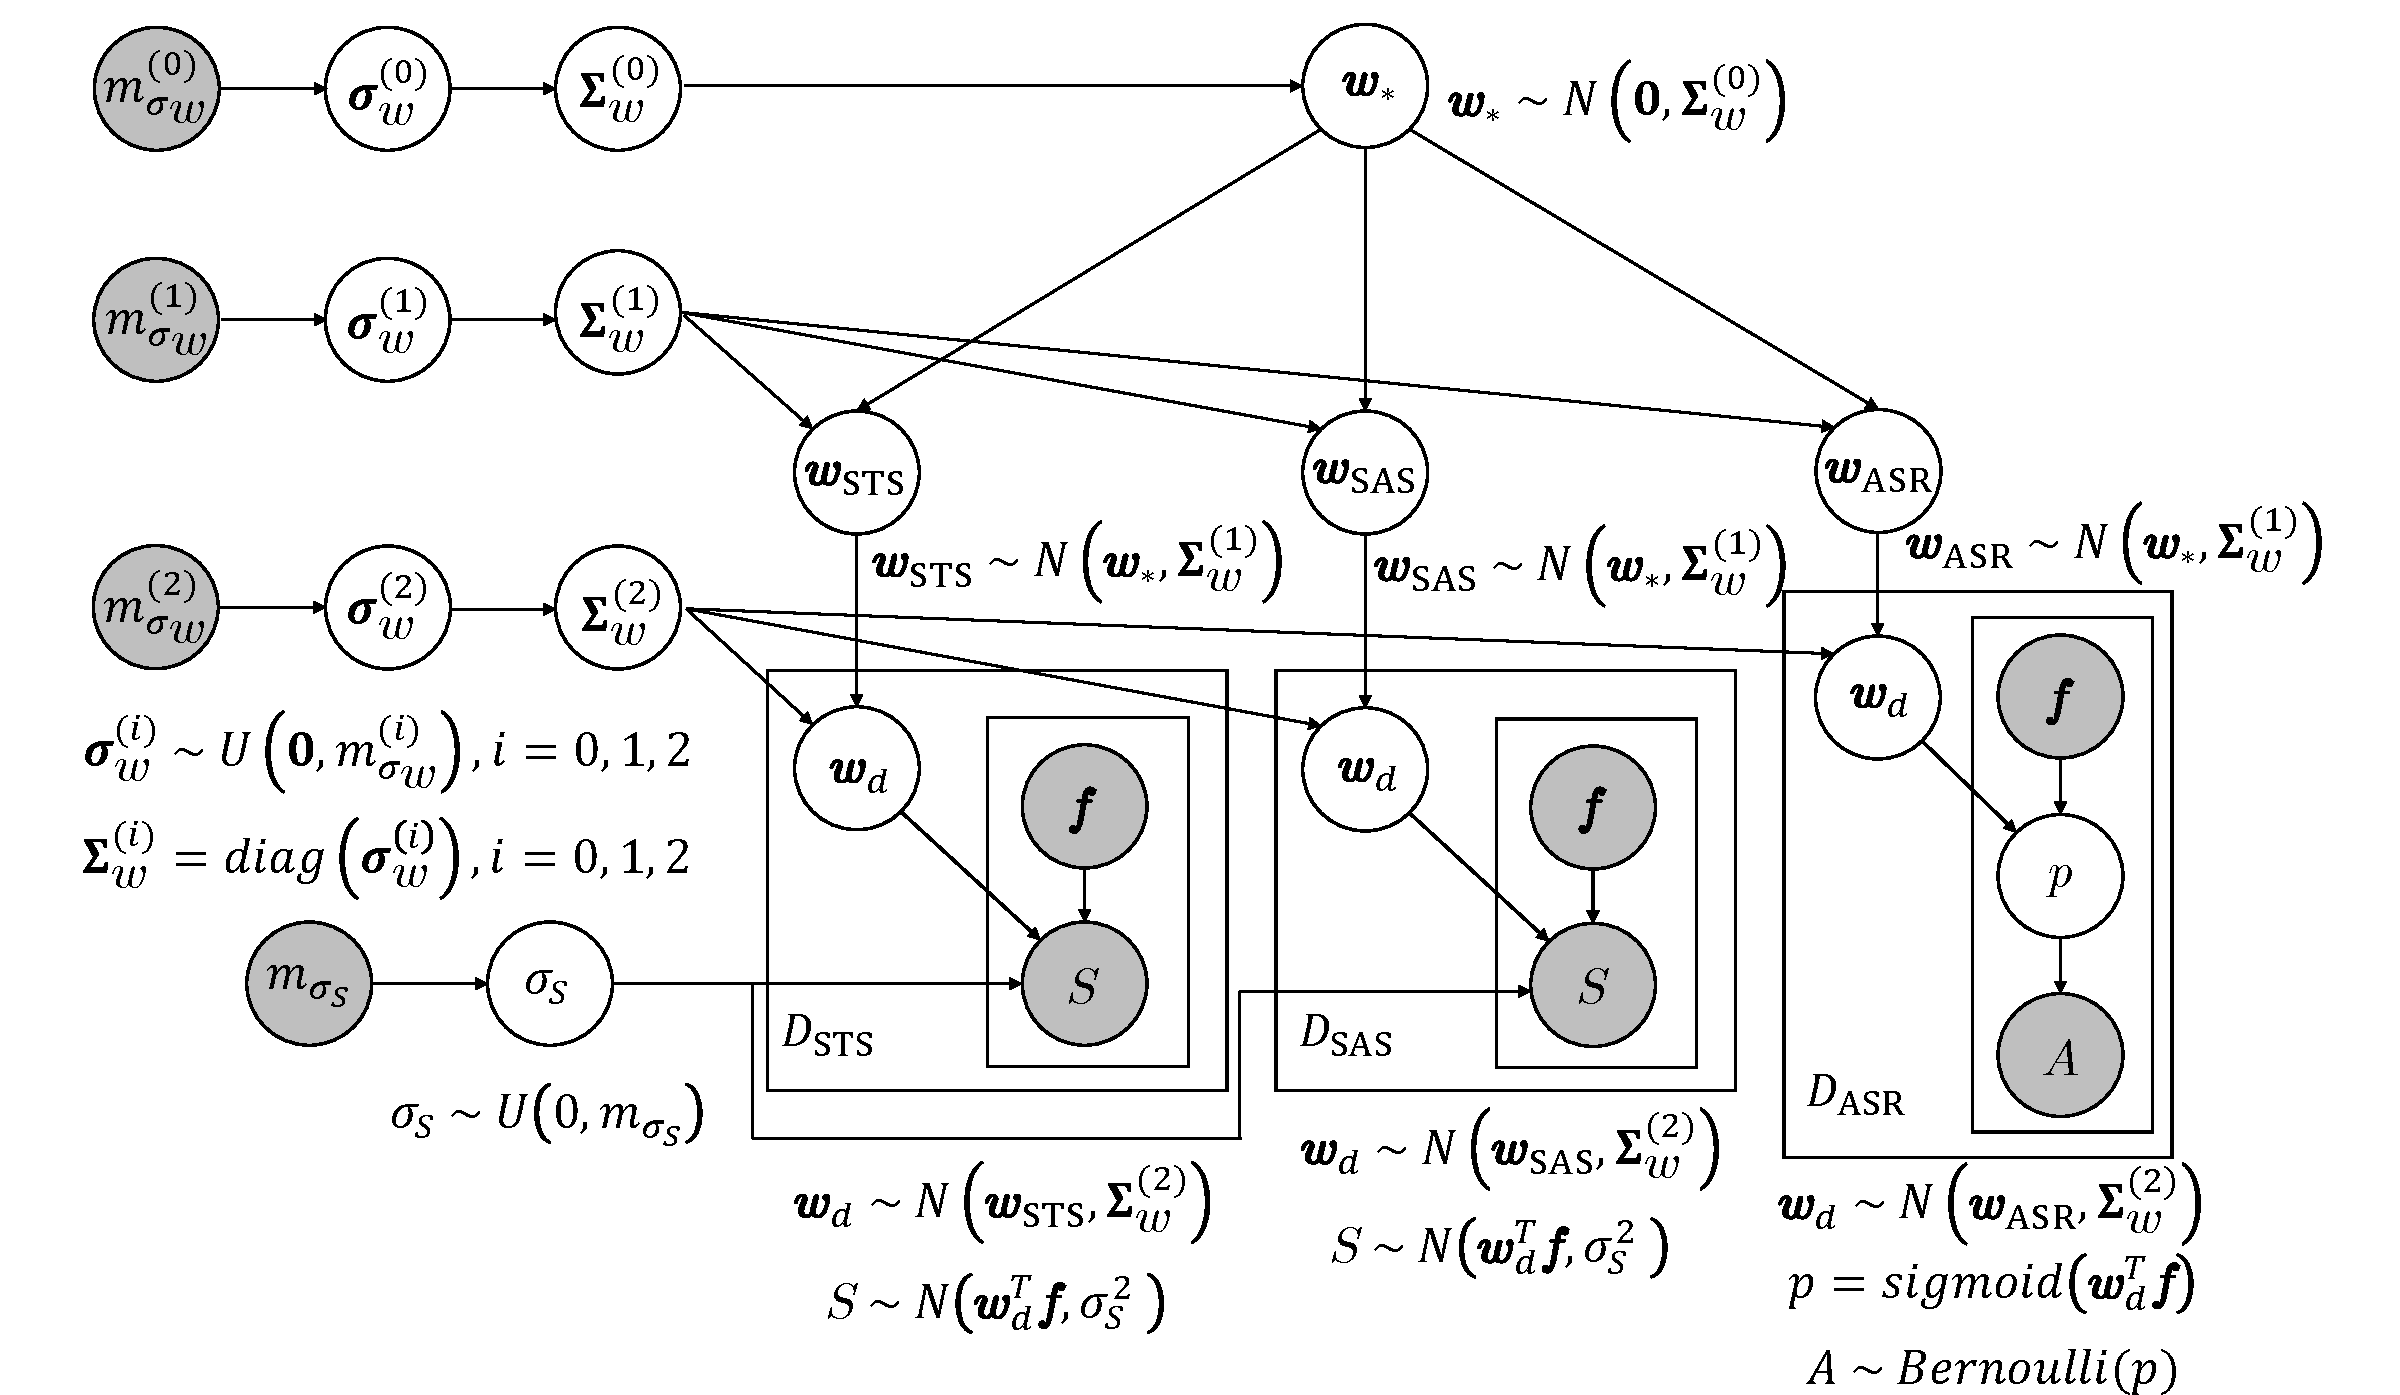
\includegraphics[scale=0.35]{2016_naacl_stsdomain/figures/three_level_da_sts_sas_qa_model_practical.pdf}
\caption{
Multitask learning: \sts{}, \sas{} and \asr{}.  Global
($\boldsymbol{w}_*$), task-specific ($\boldsymbol{w}_{\sts{}}$,
$\boldsymbol{w}_{\sas{}}$, $\boldsymbol{w}_{\asr{}}$) and
domain-specific ($\boldsymbol{w}_{d}$) weight vectors are jointly
learned, enabling transfer across domains and tasks.}

\label{figure:mtl-sts-sas-asr-model}
\end{figure*}





Each $\boldsymbol{w}_d$ depends not just on its domain-specific
observations but also on information derived from the global, shared
parameter $\boldsymbol{w}_*$.  The balance between capturing in-domain
information and inductive transfer is regulated by $\Sigma_w$; larger
variance allows $\boldsymbol{w}_d$ more freedom to reflect the domain.


\subsection{Multitask Learning}
\label{section:approach-mtl}


An advantage of hierarchical \da{} is that it extends easily to
arbitrarily nested domains.  Our multitask learning model
(\Cref{figure:mtl-sts-sas-asr-model}) models topical domains nested
within one of three related tasks: \sts{}, \sas{}, and \asr{}
(\Cref{section:tasks-and-datasets}).  This model adds a level to the
hierarchy of weight vectors: each domain-level $\boldsymbol{w}_d$ is
now normally distributed around a task-level weight vector (e.g.,
$\boldsymbol{w}_{\sts{}}$), which in turn has global Gaussian mean
$\boldsymbol{w}_*$.\footnote{We use the
same variable for the domain-specific parameter $\boldsymbol{w}_d$
across tasks to simplify notation.}  Like the \da{} model, all weights
in the same level share common variance hyperparameters while those
across different levels are separate.





Again, this hierarchical structure (1) jointly learns
global, task-level and domain-level feature weights enabling inductive
transfer among tasks and domains while (2) retaining the distinction between in-domain and
out-of-domain annotations.  A task-specific model (\Cref{figure:base-models})
that only learns from in-domain annotations supports only (2).  On the
other hand, a non-hierarchical joint model (\Cref{figure:sts-sas-asr-model})
supports only (1): it learns a single shared $\boldsymbol{w}$ applied
to any test pair regardless of task or domain.  We compare these
models in \Cref{section:experiments}.


\begin{figure}[t]
\centering
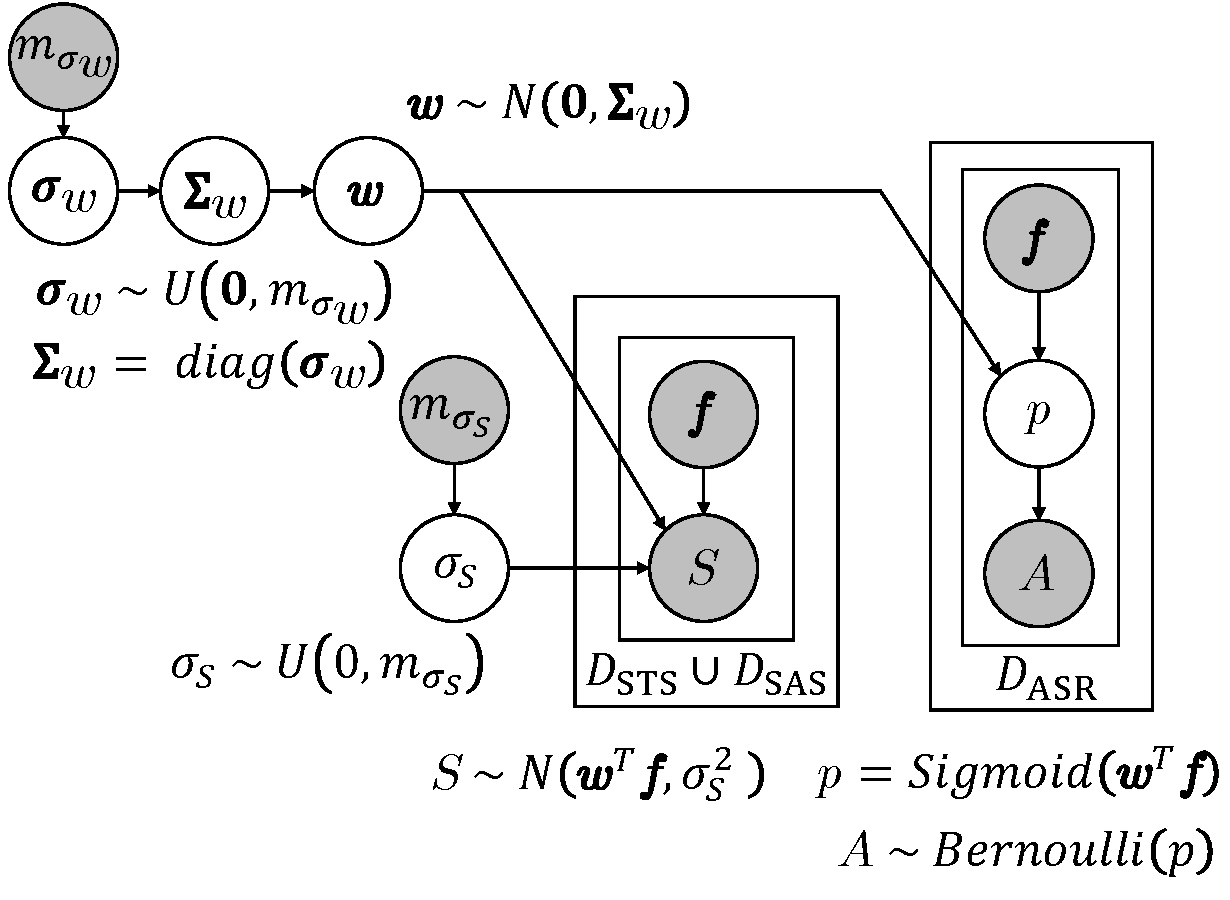
\includegraphics[scale=0.38]{2016_naacl_stsdomain/figures/sts_sas_qa_model_compact.pdf}
\caption{
A non-hierarchical joint model for \sts{}, \sas{} and \asr{}.
A common weight vector $\boldsymbol{w}$ is learned for all tasks and domains.}
\label{figure:sts-sas-asr-model}
\end{figure}










